
\chapter{Current knowledge of T cell transcriptional profiles} % Main chapter title

\label{Chapter2} % For referencing the chapter elsewhere, use \ref{Chapter1} 

%----------------------------------------------------------------------------------------

%----------------------------------------------------------------------------------------
\section{Overview}

In this Chapter we review current knowledge of how CD4$\textsuperscript{+}$ and CD8$\textsuperscript{+}$ T cells differentiate, together with an examination of the characteristic features of the resulting populations. We also discuss details of T cell activation in response to antigen presentation and how gaining a full understanding of these mechanisms is relevant to GVHD research. 

\section{Differentiation of T cell subtypes}

CD4$\textsuperscript{+}$ T helper and CD8$\textsuperscript{+}$ cytotoxic T cells are required for the generation of powerful and specific responses of the host when faced with pathogenic challenges ~\autocite{Won2016}. Both of these cell lineages develop from multipotent progenitors in the bone marrow or fetal liver. These progenitor populations subsequently go on to seed the thymus by a process of continuous migration. As precursors of the $\gamma \delta$ lineage enter the thymus, significant changes in their expression patterns of class I homeobox (HOX) genes are seen. This highly conserved family of transcription factors are indispensable for the appropriate regulation of embryogenesis and there is evidence to suggest that they may also influence T cell developmental pathways ~\autocite{Tag2003}. At the initial stage of development these T cells, known as thymocytes, are referred to as double negative (DN) by virtue of the fact that they do not express either CD4 or CD8 on their surface ~\autocite{Wee2006}. For murine lymphocytes this DN population is subdivided into three classes of maturity based upon T cell receptor expression patterns. The first group are called DN1 cells and possess the signature of CD117$\textsuperscript{+}$CD44$\textsuperscript{+}$CD25$\textsuperscript{-}$. It is noteworthy that in humans, cells at this highly immature phase of differentiation are characterised as CD34$\textsuperscript{+}$CD1a$\textsuperscript{-}$CD38$\textsuperscript{-}$ and are homologous to the DN1 cells of mice. Following some minor T cell receptor gene rearrangement, DN2 cells are formed which express CD117$\textsuperscript{+}$CD44$\textsuperscript{+}$CD25$\textsuperscript{+}$. Next, T cells characterised by CD117$\textsuperscript{-}$CD44$\textsuperscript{-}$CD25$\textsuperscript{+}$ expression are produced by major T cell receptor gene rearrangement ~\autocite{Koya2012}. These DN3 cells are further classified into two sub-populations which are referred to as DN3a and DN3b before and after $\beta$ selection respectively ~\autocite{Koya2012}. Indeed, it is the expression of T cell receptor $\beta$ that now qualifies the cells to undergo $\beta$-selection. It is at this point that cells become fully committed to the T cell lineage and begin to express CD4 and CD8 to become double-positive (DP) cells ~\autocite{Koya2012}. Interestingly Taghon \textit{et al.} observed the systematic, genomic position based down-regulation of HOX-A genes as thymic T cells increased in maturity, indicating that these transcription factors may have undetermined impacts on the differentiation of T cells subsets ~\autocite{Tag2003}. In the final stages of T cell differentiation in the thymus, triple-negative CD117$\textsuperscript{-}$CD44$\textsuperscript{-}$CD25$\textsuperscript{-}$ DN4 cells are generated which can then undergo positive and negative selection to generate mature CD4$\textsuperscript{+}$ or CD8$\textsuperscript{+}$ single-positive (SP) T cells that migrate to the periphery ~\autocite{Wee2006,Won2016,Koya2012}. This trafficking, or homing, of primed T cells primed i.e. those cells that have been activated by the primary recognition of specific peptide–MHC complexes, is required to ensure a directed, localised immune response and is primarily under the control of tissue-selective chemokines and their receptors ~\autocite{Gri2014}. The expression of adhesion molecules on the surface of migratory T cells and recognition of antigen expressed by endothelial cells also aid homing to sites of inflammation by facilitating interactions with membrane-bound integrins ~\autocite{Fu2013}. The collective expression of chemokines and adhesion molecules is sometimes used to determine the functional abilities and activation status of T cell populations ~\autocite{Won2016}. 

T cell malignancies are still prevalent worldwide and can develop at any stage of the differentiation process as well as from mature T lymphocytes in the peripheral circulation ~\autocite{Fil2002}. T-cell acute lymphoblastic leukaemia (T-ALL) for example is characterised by the abnormal proliferation of immature pre-T cell clones together with abnormal hematopoiesis and is often fatal due to the accumulation of organ infiltrates or infection ~\autocite{Tia2013}. Whilst dysfunctional T cells are a feature of T-ALL, it is currently unclear how this disease is initiated and progresses. Indeed, unlike B-cell lymphomas chromosomal translocations are only seen in a small percentage of peripheral T-cell lymphomas ~\autocite{Fil2002}. Thus, while we may possess a broad understanding of the steps involved in T cell differentiation in the thymus, there is great incentive to tackle the many questions that remain. These include, for example, quantifying the importance of Notch signalling during T cell differentiation. Notch signalling, or to give the full title the Notch signal transduction pathway, comprises a collection of highly conserved transmembrane receptors and their ligands which together influence multiple developmental processes. There are four receptors within this family, called Notch 1 to 4, which signal via the binding of a ligand on a nearby cell to the extracellular domain of the receptor protein. In mammals Jagged 1 and 2 together with Delta 1, 3 and 4 represent the known Notch ligands. This receptor-ligand interaction causes proteolytic cleavage of the Notch receptors' intracellular domain which is then free to translocate to the nucleus where it binds the transcription factor CSL and activates transcription of target genes including Hairy-Enhancer of Split (HES)1 and HES5 and Hes-related repressor protein (HERP) ~\autocite{Wee2006}. Initially, a role for Notch 1 in T cell differentiation was proposed following studies of mice with a conditional deletion of this gene in which T cell development was completely halted at the DN1 stage ~\autocite{Wee2006,Koya2012}. Notch has also been shown to be required for successful $\beta$ selection in the thymus. Furthermore, over-expression of this protein within the bone marrow was shown to induce T cell differentiation at the expense of B cell development. The involvement of Notch signalling in these cell developmental pathways is very much in keeping with the known functions of these proteins which often form part of cell-fate determining processes ~\autocite{Koya2012}. It is interesting to ponder then why other members of the Notch receptor family do not seem to play a role in the regulation of T cell development. Koyanagi \textit{et al.} obtained data suggesting that Notch 2 and 3 were expressed on the same DN thymocyte population as Notch 1 and yet their presence seems to have no direct effect ~\autocite{Koya2012}. As postulated by the authors, this finding may be the result of a differential glycosylation modification of Notch receptors by Fringe proteins ~\autocite{Koya2012,Leb2014}.

As summarised in Figure 2.1, na\"ive CD4$\textsuperscript{+}$ cells, once activated by interactions with APCs, will differentiate into one of four specialised celltypes, defined by distinct cytokine secretion, trafficking receptor expression, and the presence of a master transcriptional regulator ~\autocite{Zhu2010}, which all have critical roles in adaptive immune responses. The activation of T cells will be covered in depth elsewhere, suffice to say that the initiation of T cell differentiation requires the recognition of an MHC class II/cognate antigen complex on the surface of an APC ~\autocite{Edw2014}. Putting aside the Treg population which will be discussed later, it was originally thought that there were only two possible fates for CD4$\textsuperscript{+}$ cells, namely the Th1 and Th2 lineages ~\autocite{Awa2009}. This conclusion was based upon observations that Th1 and Th2 cells produce differing patterns of cytokines and possess distinct functions. While Th1 lymphocytes are necessary for the cell-mediated immunity against intracellular pathogens and secrete interferon-$\gamma$, lymphotoxin and IL-2, Th2 cells produce IL-4,IL-5 and IL-13 and are responsible for clearing pathogens and extracellular parasites ~\autocite{Mil2010,Awa2009, Cha2003}. Recent research has in fact challenged this classification with claims that it is too simplistic to explain the complexity of the events that lead to pathogen clearance and immune tolerance ~\autocite{Mil2010}. Indeed, there is now a great deal of evidence to support support the existence of another CD4$\textsuperscript{+}$ IL-17 secreting sub-population with unique effector function termed Th17 cells which are believed to differentiate following release of IL-23~\autocite{Awa2009}. Studies in mouse models suggest that Th17 cells are involved in defence against extracellular pathogens and that they may be implicated in inflammatory autoimmune conditions ~\autocite{Cro2009}. 

\begin{figure}[H] 
    \centering
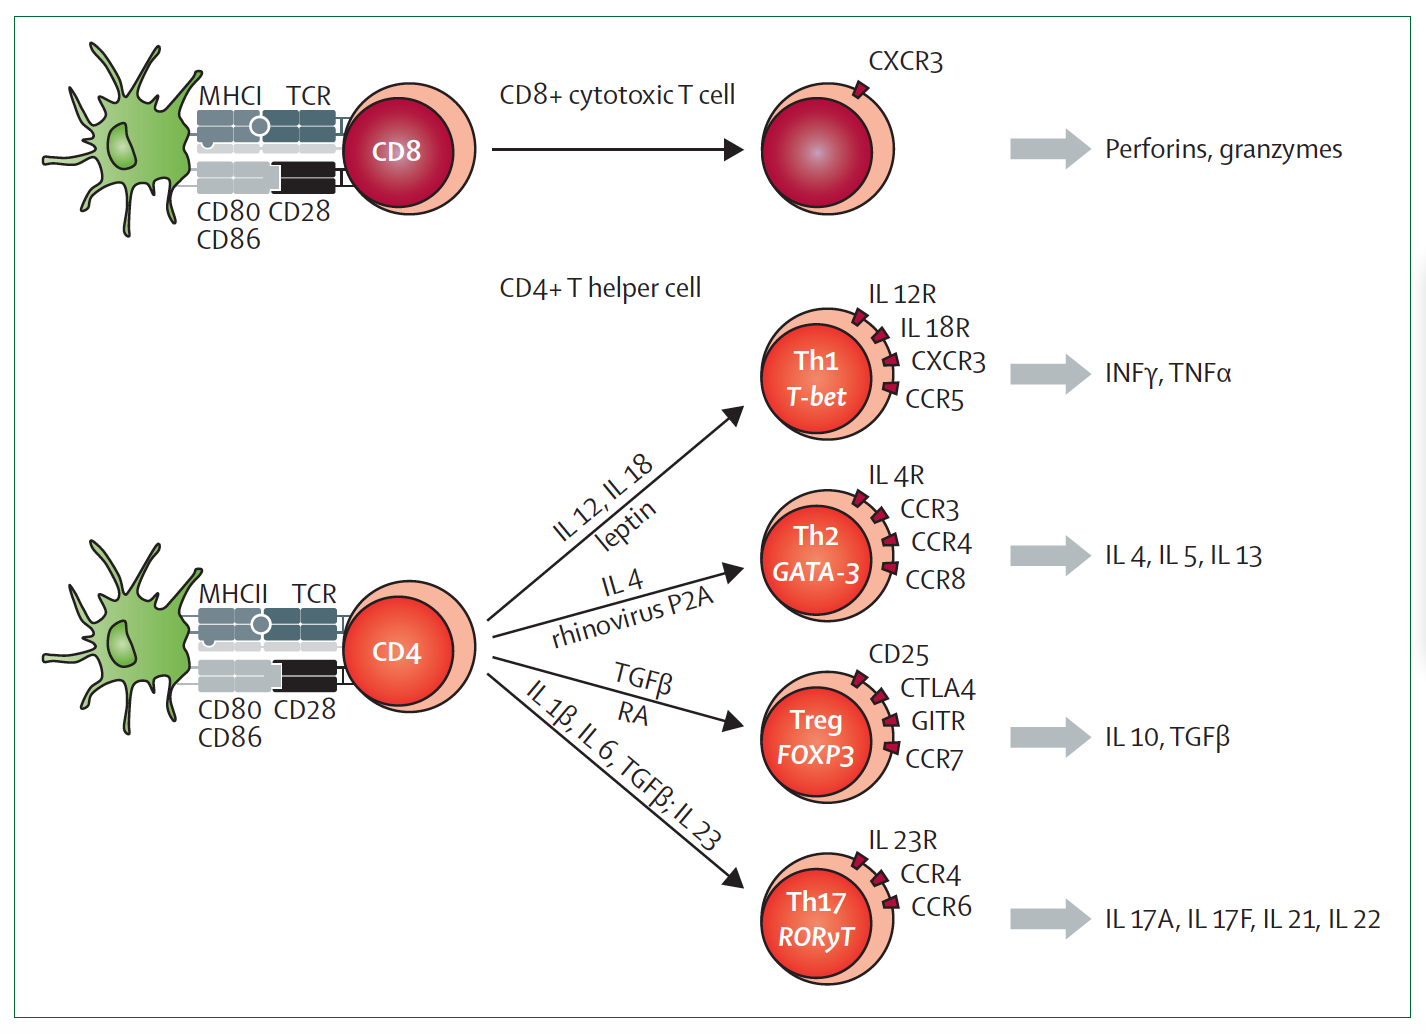
\includegraphics[width=0.8\textwidth]{Figures/Chapter2/T_cell_differentiation.png}
\caption{\small{Outline of CD4$\textsuperscript{+}$ and CD8$\textsuperscript{+}$ T cell differentiation in response to stimulation by antigen. Taken from Brusselle \textit{et al.}, 2011 ~\autocite{Bru2011}.} }
    \label{fig:6}
\end{figure}

As alluded to briefly above, it is the antigen specific activation of the T cell receptor in the presence of a polarising cytokine milieu that triggers the differentiation of T cells into a specific Th subset ~\autocite{Cha2003}. The particular lineage a cell will be committed to is additionally influenced by the concentration of antigen, strength of the TCR signal, ligation of co-stimulatory molecules, current chromatin structure and the type of APC involved in the interaction ~\autocite{Cha2003,Edw2014}. It is known that, upon antigen driven TCR stimulation, the production of Th1 cells occurs in response to the activation of Signal Transducer and Activator of Transcription (STAT)-1 and STAT-4 by IL-12 and interferon-$\gamma$ which in turn upregulate a Th1-specific transcription factor known as T-bet ~\autocite{Awa2009, Edw2014}. T-bet acts as a major player in the initiation of interferon-$\gamma$ production and hence a positive feedback loop is initiated ~\autocite{Edw2014,Tia2013}. The likely accuracy of these assertions is suggested by the observation that a deficiency in T-bet causes partial inhibition of interferon-$\gamma$ release and prevents Th1 differentiation ~\autocite{Edw2014}. Th1 cells are required for cell-mediated immune defense against intracellular pathogens and are implicated in multiple autoimmune pathologies ~\autocite{Cha2003}. These cells are also involved in the activation of CD8$\textsuperscript{+}$ CTLs and their frequency is found to be decreased in T-ALL ~\autocite{Tia2013}. It is believed that T-bet is able to influence epigenetic states of T-helper cells due to its ability to control the state of the H3K27me3 modification. This property of T-bet allows for some flexibility of the signature gene expression program of Th cells until it is extinguished ~\autocite{Mil2010}. Thus it is possible that the re-expression of this transcription factor in newly differentiated T helper cells may significantly alter their fate and effector properties. 

In contrast to the Th1 population, STAT-6 together with the transcription factor GATA-binding protein 3 (GATA-3) controls the differentiation of Th2 cells. IL-4 is the main cytokine produced by the Th2 population but the release of  IL-5, IL-6, IL-9, IL-10 and IL-13 by these cells has also been recorded ~\autocite{Cha2003}. The distinctions between the development of Th1 and Th2 lineages are highlighted by the fact that T-bet acts to repress expression of GATA-3, thus preventing differentiation of the Th2 lineage ~\autocite{Cha2003,Edw2014}. Chakir \textit{et al.} were among the first to propose that, in a population of mixed cells, the Th1 and Th2 cytokine expression patterns are best described by the T-bet/GATA-3 ratio, as against expression levels of either alone, and that GATA-3 is the more potent regulator ~\autocite{Cha2003}. It was in fact analyses of these transcription factors and STAT proteins that lead to identification of IL-17 cells as a distinct lineage as none associated with Th1 or Th2 lineages were found to be expressed by this population. Instead, human IL-17 cells are known to secrete IL-17A, TNF-$\alpha$, IL-6, CD161, IL-22 and IL-26 but are incapable of producing interferon-$\gamma$ ~\autocite{Cro2009}. Even more convincingly, TGF-$\beta$, which along with IL-6, IL-21 and IL-23 is important for the specialisation of TH17 cells \textit{in vivo} via induction of phospho-STAT3, actually inhibits T-bet and GATA-3, thereby preventing differentiation of both Th1 and Th2 populations ~\autocite{Awa2009,Sch2014}. Another feature which sets Th17 cells apart from Th1 and Th2 populations is a lack of self-amplification abilities. Th1 cells are amplified by a positive feedback loop involving IFN-c, STAT-1 and T-bet, while IL-4 fulfils a similar role in in the case of Th2 cells. IL-17 on the other hand is not a differentiation factor and its receptor is not expressed on T cells ~\autocite{Awa2009}. There was some discussion of whether IL-23 might be the primary differentiation factor for Th-17 cells but this was later dismissed due to incompatible expression patterns and a lack of experimental evidence and so debate continues over the precise cytokine activity that optimally induces the development of Th-17 cells ~\autocite{Cro2009}. TGF-$\beta$ and IL-6 have been demonstrated as helping to polarise na\"ive CD4$\textsuperscript{+}$ T cells into Th17 cells in mice, while IL-23 is thought to be required for the expansion, maintenance and effector function of this population ~\autocite{Cro2009, Awa2009, Sch2014}. Although some early studies suggested that TGF-$\beta$ actually had an inhibitory function on Th17 cell differentiation, later work produced countering results ~\autocite{Awa2009}. The requirement for TGF-$\beta$ in the successful differentiation of Th17 cells is therefore still debated, as is the cellular source of this factor which can be produced by multiple leukocyte lineages. What is known is that the successful differentiation of Th17 cells requires the actions of multiple transcription factors. As well as STAT-3 which has already been mentioned, Ror-$\gamma$ t, Ror-$\alpha$ and interferon-regulatory factor 4 all play a part ~\autocite{Cro2009}. Once fully specialised, it is the production of the inflammatory cytokine IL-17 itself that is believed to be crucial for many effector functions of Th17 cells including maintaining mucosal barriers and the efficient clearance of pathogens/fungal infections ~\autocite{Cro2009,Gau2015}. In addition, IL-17 is responsible for the stimulation of cytokine and chemokine release from numerous celltypes and can also assist in the recruitment of neutropils to sites of inflammation. Dysregulation of Th17 effector response can cause dangerous levels of tissue inflammation in the host ~\autocite{Awa2009}. Interestingly, Wong \textit{et al.} comment that in their recent analysis they identified Th cells capable of secreting multiple Th cell-associated cytokines, e.g. cells producing  IFN-$\gamma$, IL-17, and IL-22 simultaneously ~\autocite{Won2016}. 

Regulatory T cells (Tregs), usually subdivided into natural Tregs (nTregs) and adaptive or induced Tregs (iTregs), are circulating CD4$\textsuperscript{+}$ cells well known as being able to suppress both physiological and pathological immune responses. Indeed, a deficiency of Tregs leads to serious systemic autoimmunity ~\autocite{Sch2014}. Focusing on involvement with malignant tumours, it has been seen that Tregs localise to the vicinity of the the damaged tissue which they may be attracted to by chemokine release from the tumour itself. For example, some tumours secrete the chemokine (C-C motif) ligand 22 (CCL22) which is recognised by the chemokine (C-C motif) receptor 4 (CCR4), that is expressed on the surfaces of Tregs in high concentrations ~\autocite{Sch2014}. Tregs are selected in the thymus based on high-avidity interactions and nTregs comprise between 5 and 10\% of total CD4$\textsuperscript{+}$ cell counts ~\autocite{Sch2014}. These cells are characterised by their expression of forkhead box P3 TF (Foxp3). There is evidence that TGF-$\beta$ is important for the differentiation of Foxp3$\textsuperscript{+}$ nTreg cells from naive CD4$\textsuperscript{+}$ T cells as well as maintenance of their functional capabilities ~\autocite{Awa2009}. It has been proposed that nTregs are formed in the thymus in a two-step process. Initially Treg precursors are generated which requires factors such as CD-28 and various cytokine receptors and this is then followed by the binding of IL-2 to its receptor and the resulting expression of Foxp3 ~\autocite{Sch2014}. It is interesting to note that low concentrations of TGF-$\beta$ promote Foxp3 expression, thereby favouring Treg differentiation, while at high levels TGF-$\beta$ induced upregulation of the IL-23 receptor leads to the IL-17 phenotype ~\autocite{Sch2014}. IL-2 has also been shown to activate the tumour effects of NK cells ~\autocite{Tia2013}. The fact that Th17 and Treg cells undergo mutually exclusive differentiation pathways may indicate that they share a common T cell precursor that can differentiate into either celltype depending on the particular milieu of cytokines present ~\autocite{Awa2009}. It has been shown that TGF-$\beta$ plays an additional role in nTreg differentiation by protecting immature cells from apoptosis via the upregulation of Bcl-2 which promotes cell survival, as well as suppressing pro-apoptotic proteins ~\autocite{Sch2014}. 

The final population to arise from T cell differentiation are the CD8$\textsuperscript{+}$ cytotoxic T lymphocytes (CTLs). These cells are essential for immunity to both viral and bacterial pathogens. During infection or following immunisation, a small number of na\"ive CD8$\textsuperscript{+}$ cells are activated by interactions with their cognate antigen, after which they undergo rapid clonal expansion and further differentiation to become killer CTLs ~\autocite{Gra2014,Roy2015}. It is believed that this process of specialisation involves differential patterns of gene expression brought about by epigenetic modifications, such as alterations to DNA methylation states and remodelling of the chromatin structure, which are themselves regulated by cytokine activity and T cell receptor signalling. Killer CTLs are able to neutralise target pathogen via the secretion of molecules including granzyme and IFN$\gamma$. Once the pathogen in question has been successfully cleared most of the effector CTLs die leaving only a few remaining in the circulation. The fate of those cells that survive is to become memory CTLs whose role it is to promptly clear pathogens to which the individual has already been exposed, thus avoiding another primary adaptive response by the immune system and preventing a second full-blown infection ~\autocite{Roy2015}. Upon secondary infection memory cells quickly expand, producing a response that is often more effective than during initial exposure ~\autocite{Roy2015}. A person will be deemed as possessing immunologic memory when their memory CTLs are still present at least 1 month post-infection ~\autocite{Gra2014}. It is at this time point that the memory CTLs are uniquely able to undergo homeostatic proliferation upon the release of IL-7 and IL-15.  The importance of the PI3K/AKT/ mTOR axis for the differentiation of cells with memory CTL phenotype has been emphasised and epigenetic factors are again likely to be important although the specific nature of the remodelling, should it indeed occur, is still not clear ~\autocite{Gra2014,Edw2014}. There is additional evidence that the differentiation of na\"ive CD8$\textsuperscript{+}$ T cells to CTLs is partially regulated by Notch signalling pathways but this is yet to be investigated fully ~\autocite{Koya2012}. It is important to note that due to variations in factors such as duration of antigen stimulation, levels of inflammation and antigen-specificity there is a great deal of heterogeneity in the specific effector and memory CTL populations that are produced during a given infection. Following studies examining the antiviral responses of mice there are now two models, called linear and progressive differentiation, to explain predominance of effector cells during acute phases of the response and cells with a memory phenotype at later phases. The linear differentiation hypothesis states that upon antigen interaction na\"ive CD8$\textsuperscript{+}$ T cells always differentiate into effector cells which then either undergo apoptosis or further differentiate into central/effector memory T cells which persist once the pathogen is cleared \autocite{Roy2015}. Alternatively, it is thought CD8$\textsuperscript{+}$ T cells may differentiate following a single path from na\"ive state to central memory, effector memory and lastly effector phenotype. This progressive differentiation model additionally suggests that the changes occurring at each phase are irreversible ~\autocite{Roy2015}. Despite multiple studies in this field, there are findings to support each of these CD8$\textsuperscript{+}$ T cell lineage differentiation theories. Indeed, while one group utilising an artificial Gzmb promoter sequence found that T cells that had previously been effectors could contribute to the memory pool, Kaech \textit{et al.} were able to demonstrate that effector cells had a reduced capacity for forming memory cells ~\autocite{Kae2003,Roy2015}. In their work, Roychoudhuri \textit{et al.} observed that central memory cells were transcriptionally more similar to na\"ive CD8$\textsuperscript{+}$ cells than were effector or effector memory populations, a finding which fits with a model of progressive differentiation resulting from cumulative antigen exposure ~\autocite{Roy2015}. It has also come to light in recent years that humans may possess an additional memory T cell subtype which is now commonly referred to as the stem-cell memory like (TSCM) population ~\autocite{Edw2014}. T cells with this phenotype are multipotent with the capacity to become either central memory, effector memory or effector T cells as well as enhanced self-renewal abilities.

\section{Subtype characteristics}

There is still much to understand when it comes to the details of T cell biology, but current evidence from post-mortem analyses indicates that there is distinct tissue specific compartmentalisation of both subset populations and their associated trafficking receptors that is seemingly conserved irrespective of the age, cause of death or racial background of the patient ~\autocite{Won2016}. The shear number of studies examining the specific features of differentiated T cell populations means we possess increasing insight into what characteristics are descriptive of a given subtype. CD4$\textsuperscript{+}$ cells as already mentioned evoke a wide range of effector functions and are necessary for the elimination of both extracellular and intracellular pathogens. Through the process of differentiation upon activation, CD4$\textsuperscript{+}$ Th cells are able to perfect and maintain their antigen specific effector functions, including proliferation, cytokine production and lysing of target cells, which facilitates a fast and powerful immune response if re-exposure should occur ~\autocite{Edw2014}. The classification of CD4$\textsuperscript{+}$ Th subsets based upon cytokine and transcription factor expression profiles has already been discussed in some detail. However, in addition to T-bet expression and interferon-$\gamma$ secretion, there is another protein which is characteristic of Th1 cells. Eomesodermin (Eomes) is a T-box transcription factor whose expression on CD4$\textsuperscript{+}$ T cells arises following stimulation of TCRs and the resulting upregulation of T-bet ~\autocite{Edw2014}. Eomes expression is not thought to be capable of altering the differentiation paths of other Th cell lineages, but it can promote interferon-$\gamma$ production and has been shown to assist in the process of Th1 fate determination alongside T-bet. Edwards \textit{et al.} showed in a recent study that CD4$\textsuperscript{+}$ cells adjust their cytokine and T-box transcription factor expression patterns depending on the nature of the antigen presented to them during infection, thus demonstrating marked levels of functional plasticity ~\autocite{Edw2014}. To further highlight this modulation of T cell transcriptional profiles, Edwards \textit{et al.} exposed CMV-specific CD4$\textsuperscript{+}$ T cells to various CMV antigens with quite interesting results. When challenged with the CMV proteins pp65 and gB, CD4$\textsuperscript{+}$ cells were mostly interferon-$\gamma\textsuperscript{+}$ TNF-$\alpha\textsuperscript{+}$ in phenotype, while cells specific for the IE-1 CMV peptide expressed TNF-$\alpha$ in isolation ~\autocite{Edw2014}. Furthermore, this group found that the levels of cytokine production were higher in the double positive population than for the single positive cells. These two distinct T cell groups also expressed differing proportions of T-bet and Eomes which may indicate that these transcription factors are together involved in modulating the functional properties and effector functions of antigen specific immature T cells during an immune response ~\autocite{Edw2014}. Antigen load is likely to be a key variable in the differentiation of CD4$\textsuperscript{+}$ T cells with this amount of flexible functionality, as is known to be the case in the generation of CD8$\textsuperscript{+}$ memory T cells. There is thus some evidence at least of heterogeneity within CD4$\textsuperscript{+}$ T cell sub-populations produced in response to some infections including CMV. This is a particularly tantalising prospect from a clinical prospective as periodic reactivation of viruses such as CMV can lead to T cell exhaustion and resulting loss of effector functions. If Edwards \textit{et al.} are correct, less differentiated T cells may potentially be able to step into the breech and specialise in order to successfully upregulate effector functions and control the infection ~\autocite{Edw2014}. 

Turning to the IL-17 producing CD4$\textsuperscript{+}$ population, it has been demonstrated that polarisation of these cells \textit{in vitro} with IL-1, IL-23 and IL-6 can lead to intense autoimmune pathology on some occasions and yet may have no effect on others ~\autocite{Gau2015}. Furthermore, IL-17 cells, which are generally considered to be an early subset of effector cell, have been observed as adopting varying phenotypic states as they travel through the lymphatic and central nervous systems ~\autocite{Tia2013,Gau2015}. Beginning with a self-renewing phenotype in the lymph nodes, Th-17 cells seem to adopt a pre-Th1 effector-like phenotype as they migrate to the central nervous system (CNS). These CD4$\textsuperscript{+}$ cells have been seen to emulate a Th1-like effector state and a Th1-like memory state whilst in the CNS before eventually losing some of their functionality. It is likely that the effector phenotype identified in the CNS is the most pathogenic and may allow for the formation of memory cells as occurs in Th1 populations. There is evidence that Th17 cells in the CNS are regulated by transcription factors such as Hif1a, Fosl2, Stat4, and Rel which are already known to be involved in Th1 and Th17 cell fate determination. Researchers have been able to characterise the self-renewing Th-17 cells in the lymph nodes and they were found to possess a Wnt signalling signature with high expression of a key Wnt target and transcription factor, Tcf7 ~\autocite{Gau2015}. These cells also upregulate the na\"ive cell marker Cd62l and the pro-survival gene Cd27. Gaublomme \textit{et al.} postulate that the transcription factors Med12, Etv6, and Zfx are probable regulators of this population of potential Th17 effector/memory precursor cells ~\autocite{Gau2015}. It is currently unclear whether these Th17 cells are simply able to "mimic"  their Th1 cousins in addition to their own characteristic phenotype, or whether they are demonstrating plasticity towards a change in cell fate. Considering the involvement of Th17 cells in both functional haematopoiesis and autoimmune/inflammatory diseases, this latter possibility is extremely intriguing and worthy of further investigation ~\autocite{Tia2013}.  

If choosing to classify T cell subtypes based on their cytokine and chemokine profiles, some would argue the existence of an additional CD4$\textsuperscript{+}$ subset characterised by IL-22 production and CCR10 expression. IL-22 acts via a heterodimeric transmembrane complex comprised of IL-22R1 and IL-10R2 and is also known to signal through activators of transcription (JAK-STAT) pathways and subsequent Janus kinase-signal transducers. So called Th22 T cells are believed to differentiate as a result of the activities of transcription factor AHR and do not express either IL-17, CD161 or interferon-$\gamma$ thus setting them apart from other CD4$\textsuperscript{+}$ populations ~\autocite{Tia2013}. These cells share expression of chemokine (C-Cmotif) receptor 6 (CCR6) and CCR4 with the Th17 subset, but this is the entirety of any functional overlap. Furthermore, expression of  T-bet and RORC, known in transcription factors for the Th1 and Th2 lineages as described earlier, is virtually non-existent in Th22 populations. Putting these findings together with potential involvement in inflammatory and autoimmune pathologies ~\autocite{Tia2013}, it can be seen that there is substantial evidence to support the definition of Th22 T cells as a fully differentiated, functional Th subset. 

Quantitative analyses of CD8$\textsuperscript{+}$ subtype transcriptional profiles have revealed the expression of unique patterns within each population. Putting aside the comparatively few unique elements, Roychoudhuri \textit{et al.} made the surprising discovery that when considering differentially expressed genes before and after vaccination regimens in mice, central memory CD8$\textsuperscript{+}$ T cells were more similar in terms of transcriptional profiles to na\"ive cells than to either effector or effector memory populations ~\autocite{Roy2015}. These findings were echoed in multidimensional scaling analysis. The differentially expressed genes were analysed using unsupervised hierarchical cluster analysis to help elucidate potential mechanisms underlying the these observations and a total of six clusters were identified. Interestingly, the two largest gene clusters - named A and B - exhibited changes in expression which were progressively up- or down-regulated in line with the differentiation state of the population ~\autocite{Roy2015}. Cluster A contained transcription factors such Tbet and Id2 as well as genes associated with T cell senescence while markers of T cell longevity and the lymphoid homing molecule CD62L were grouped within cluster B. The other clusters produced were significantly smaller and exhibited fluctuations only in one or two CD8$\textsuperscript{+}$ T cell subtypes ~\autocite{Roy2015}. By comparing their observed global transcriptional differences between CD8$\textsuperscript{+}$ T cell subset populations with those defined by Wirth \textit{et al.} in a study of the effects of repeated (primary, secondary, tertiary or quaternary) antigen stimulation ~\autocite{Wir2010}, Roychoudhuri \textit{et al.} identified multiple correlations between the two datasets ~\autocite{Roy2015}. Central memory cells were transcriptionally most similar to T cells exposed to antigen only once, while those experiencing secondary stimulation shared the greatest transcriptional overlap with effector memory CD8$\textsuperscript{+}$ T cells. Finally, the characteristic transcriptional signal of effector cells was most akin to that of CD8$\textsuperscript{+}$ T cells following quaternary antigen stimulation ~\autocite{Roy2015}. There is evidence therefore that CD8$\textsuperscript{+}$ T cells differentiating following vaccination can possess the transcriptional imprint of differential exposure to antigen. Roychoudhuri \textit{et al.} subsequently focused on the expression patterns that were characteristic of each subtype. The gene encoding Cxcr5, which is known to help CD8$\textsuperscript{+}$ T cells travel to the lymph nodes, was enriched in central memory cells as was Xc11 which is involved in ensuring proper interactions between T cells and dendritic cells ~\autocite{Roy2015}. Within the effector memory populations the chemokine receptors Ccr5 and Cxcr6 were up-regulated, whilst the effector CTL cells showed high levels of the Slamf1 leukocyte cell-surface glycoprotein that is implicated in cell death following activation and T cell receptor signalling ~\autocite{Roy2015}. 

A recent study by Mackay \textit{et al.} identified two key genes, Hobit (Zfp683) and Blimp1 (Prdm1), which, aside from roles in the maintenance of NK cell populations, the authors believe have specific expression profiles in tissue resident memory of (Trm) CD8$\textsuperscript{+}$ T cells ~\autocite{Mac2016}. The role of these cells, which are characterised by the dual expression of activation marker CD69 and trafficking receptor CD103 ~\autocite{Tho2015}, is to facilitate immediate protection in case of reinfection and as such they migrate to - and remain at - sites of pathogen entry. This group analysed the expression patterns of Trm CD8$\textsuperscript{+}$ cells following infection with herpes simplex virus (HSV) or lymphocytic choriomeningitis virus (LCMV) and saw substantial differences in expression depending upon the tissue examined. In skin both Hobit and Blimp1 expression patterns changed following infection, but in opposite directions. T cell expression of Hobit, which is known to be under the transcriptional control of T-bet, was seen in skin cells alone and gradually increased until 30 days post infection. Blimp1 on the other hand was expressed in populations of CD8$\textsuperscript{+}$ T cells resident in the spleen and skin with levels peaking early at day 8 post infection ~\autocite{Mac2016}. Characteristic expression profiles in memory CD8$\textsuperscript{+}$ T cells observed following lymphocytic choriomeningitis virus (LCMV) followed a similar path with ubiquitous Blimp1 induction and gut specific expression of Hobit. It seems evident from these results that in the case of CD8$\textsuperscript{+}$ T cells, Hobit expression is Trm location specific but knock-out studies would indicate that Blimp1 is also involved in the development and functionality of tissue-resident lymphocytes. Expression patterns comparable to those outlined here have been identified in the NKT1 subset of invariant natural killer T (NKT) cells which also depend on T-bet, suggesting that  that the mechanisms involved in driving tissue residency are likely to be conserved between T lymphocyte populations ~\autocite{Mac2016}. Blimp1 and Hobit possess highly homologous DNA-binding zinc finger domains and so to better understand their input in influencing tissue residency, Mackay \textit{et al.} performed both gain and loss of function experiments highlighting their impact on expression levels of many genes before attempting the identification of potential binding sites ~\autocite{Mac2016}. Over 50\% of the genome-wide binding sites identified for Hobit overlapped with those of Blimp1, supporting the notion that these two factors act together to mediate the transcriptional programs of Trm T cells. In a study characterising T cell subtypes found in the human body, Thome and Farber identified Trms in all tissues surveyed with the exception of blood ~\autocite{Tho2015}. In their study Thome and Farber isolated four Trm subtypes within the CD8$\textsuperscript{+}$ T cell compartment, three expressed at high levels in the colon, two of which were also seen in the lung, and a final population localised to the spleen and tonsils ~\autocite{Tho2015}. These populations exhibited differences in both function and expression of markers including CD103, CD45RO and CCR5, thus highlighting the phenotypic variation evident in different human CD8$\textsuperscript{+}$ Trm populations. 

\section{Activation of T cells}

It has long been recognised that the appropriate functioning of the immune system is reliant upon the appropriate differentiation of both T and B cell receptor repertoires as well as regulation of response phases namely commitment, expansion, and contraction ~\autocite{Bur2015}. The processes of T cell differentiation and proliferation into well defined subsets are triggered in response to the recognition of antigen and it is this mechanism that will be described in depth here. 

Numerous cell types have been shown to play a part in the presentation of antigen to na\"ive T cells with varying efficiencies. These include both hematopoietic and non-hematopoietic populations which together are called antigen presenting cells (APCs) ~\autocite{Cha2007}. An adaptive immune response will only be initiated if the amount of antigen processed and presented by these populations reaches a certain threshold. Once antigen has been processed by the cell, the corresponding peptides can be loaded onto major histocompatibility complex (MHC) molecules before being delivered to the cell surface as composite structures with co-stimulatory and adhesion molecules ~\autocite{Cha2007}. In conjunction with one another, these components assist in the formation of an immunological synapse with a T cell. Professional APCs, including dendritic cells (DCs), B cells and macrophages, are hematopoietic lineages that have specialised specifically to take up, process and present antigen and they execute their task with high efficiency. It is possible for some other cell types to acquire antigen-presenting capabilities in particular circumstances and this phenomenon has been demonstrated in T cells, type 2 innate lymphoid cells (ILC2s), CD34 progenitors and non-hematopoietic populations alike ~\autocite{Bur2015,Cha2007,Igy2013}. Despite being heavily influenced by origin and activation history, DCs have been shown to be the most powerful APC population when it comes to priming na\"ive T cells and they are also able to take up antigen from peripheral tissues and transport it to the secondary lymphoid organs. 

It has been established that separate pathways have evolved for the loading of peptides onto MHC molecules. In the case of MHC class I the endogenous pathway is followed whereby proteins or peptides within the cytosol are degraded by the proteasome and then subsequently translocated to the endoplasmic reticulum where they are loaded onto MHC molecules ~\autocite{Cha2007}. MHC class II peptides on the other hand are loaded via exogenous mechanisms involving the uptake of soluble or particulate antigens by phagocytosis. The antigens are then hydrolysed by peptidases before the derived peptides are loaded onto the MHC molecule within the endolysosomal system. Some APC populations such as murine CD8$\textsuperscript{+}$ DCs are actually capable of altering the processing fate of certain antigens from the exogenous to the endogenous pathway via a process that is known as cross-presentation ~\autocite{Cha2007}. In such situations DC, or DC progenitor, populations may traffic antigen to the lymph nodes from peripheral tissues, thus delivering them to cross-presenting CD8$\textsuperscript{+}$ DCs ~\autocite{Igy2013}. CD8$\textsuperscript{+}$ DCs, which have been identified in mice lymphoid tissues and express CD8 $\alpha$ as well as a unique combination of other surface molecules, are key players in promoting CD8$\textsuperscript{+}$ T cell responses via the prolific presentation of pathogenic antigen ~\autocite{Sho2010}. It is thought that antigen cross-presentation by such cells is required for the proper acquisition of immunity to some tumours and infectious pathogens ~\autocite{Cha2007}.

When considering the initiation of GVHD there remains debate regarding whether the presentation of minor histocompatibility antigens within class I and class II MHC complexes can both trigger Graft-versus-Host pathologies ~\autocite{Tou2012}. While it has been shown that antigen presentation by MHC class I on recipient hematopoietic APCs is necessary for the initiation of CD8$\textsuperscript{+}$ T cell-dependent acute GVHD, whether expression of allogeneic peptides in complex with MHC class II on donor or host APCs can also induce this disease is still uncertain ~\autocite{Koy2012}. Indeed, while one study did report the initiation of CD4$\textsuperscript{+}$ dependent GVHD by MHC class II expressing APCs, the study did not analyse MHC peptides and instead focused on a model in which only conformational changes in the whole MHC molecule can be recognised by T cells and so the results are not as comprehensive as they might otherwise be ~\autocite{Koy2012,Tes2002}. Following HSCT and the associated pre-transplant conditioning regimens, the APC environment is dramatically disrupted. Indeed, while some populations such as the macrophage and skin DC compartments seem comparatively resistant to this myeloablative conditioning, host radio- or chemo-sensitive APC and precursor populations are completely lost within the first few days post-transplant ~\autocite{Cha2007}. Current research indicates that differentiated APCs within the donor graft or populations differentiating from donor progenitor cells subsequently fill this void. Indeed, it was shown many years ago that host bone marrow derived cells, most likely APCs expressing class II alloantigen, were not always required for the initial retention of CD4$\textsuperscript{+}$ or CD8$\textsuperscript{+}$ T cells within the lymph nodes ~\autocite{Kos1993}. Whilst the number of host DCs able to survive the conditioning process and prime/activate effector T cells is believed to be small, it has been found that donor APCs transferred with the graft or or those developing from hematopoietic progenitor cells do not contribute to the initiation of GVHD, thus indicating that host APCs are likely to play a role, however small a population they may be ~\autocite{Cha2007}. Although their involvement in GVHD initiation is unlikely, donor APCs may be responsible for perpetrating tissue injury via the cross-presentation of host antigens and the presentation of IL-15 and its receptor on their surface. The anti-apoptotic functions of IL-15 are partially responsible for the activation of CD8$\textsuperscript{+}$ T cells and the maintenance of memory CTL populations. Despite these claims, early research conducted in mice who lacked MHC class I expression on their APC populations, revealed that such mice were resistant to GVHD pathologies ~\autocite{Shi1999}. This data would suggest that cross-priming of CD8$\textsuperscript{+}$ T cells is insufficient for the initiation of GVHD in mice, but whether this is an accurate assertion remains to be conclusively proven.

The relevance of bacterial leakage caused by conditioning regimens and resulting cytokine release to GVHD tissue injury has been discussed previously (see Chapter \ref{Chapter1}.1.4), however it has also been shown that DC populations are particularly sensitive to the presence of microbial products due to their expression of pattern-recognition receptors such as Toll-like receptors (TLR). There is evidence that triggering of TLRs in combination with adaptive immune responses is necessary for the full "licensing" of DCs which are then capable of effectively priming T cell responses, although the precise requirement of this process for the establishment of GVHD pathologies is not yet known ~\autocite{Cha2007}. The fact that GVHD is seen in both a Myd88 knock-out system, where host APCs cannot respond to effectively to TLR signals, as well as in CD40 knock-out mice who possess APCs that cannot be activated by donor T cells, indicates that there must be considerable redundancy in the requirements for APC activation. It may be that external factors such as inflammation may bypass the need for the activation of certain pathways or even the involvement of CD4$\textsuperscript{+}$ T cells ~\autocite{Cha2007}. However it is enforced, it seems likely that APC "licensing" is of significant importance in the development of tissue specific GVHD injury and furthermore, that this process can overcome the regulatory mechanisms that induce peripheral tolerance. As discussed by Chakraverty and Sykes in their review of this research theme, separate mechanisms may govern this APC "licensing" depending on the timing of GVHD induction post-HSCT ~\autocite{Cha2007}. Immediately post-transplant the release of effector T cell specific proinflammatory cytokines including IL-6, by DC populations together with the depletion of host Tregs may be sufficient to override any regulatory mechanisms employed by the host. At later time points a reduction in inflammation precedes development of a new "steady state" where few host APCs remain and those that do are deactivated. In this setting where APC activation is absent, tolerance is induced by the abortive proliferation of specific T cells that lack the capacity to generate effector cytokines in response to specific antigen presentation by DCs ~\autocite{Cha2007}. This theory is supported by experimental work in murine models of GVHD where the transfer of donor T cells immediately post-transplant can lead to GVHD pathology as well as GVL, while if the transfer of T cells is delayed by approximately one month virtually all Graft-versus-Host reactivity is lost suggesting that the immune response to such infusions lessens over time. 

Langerhans cells (LC) represent the only DC population to reside in the epidermis and are also found in the mucosal epithelia ~\autocite{Igy2013,Kis2005}. Given their location in barrier tissues, they are one of the first populations to interact with pathogens, commensal organisms and foreign chemicals and there is much evidence to suggest that LCs can transport the antigens they encounter to regional lymph nodes where they present to na\"ive T cells, initiating cutaneous immune responses ~\autocite{Igy2013}. The precise involvement of LCs in the initiation and development of GVHD is still the subject of much debate. Over a decade ago, results of GVHD studies undertaken in mice suggested that LCs were responsible for cutaneous GVHD ~\autocite{Mer2004}, but other studies have produced contradicting findings ~\autocite{All2003,Car2004}. Much of this debate concerns whether or not LCs are able to cross-present antigen. As summarised by Igyarto and Kaplan there have, to date, been three primary approaches to examine the cross-presenting abilities of LC populations ~\autocite{Igy2013}. The first and perhaps most convincing of these involves the \textit{in vitro} generation or isolation of LC from tissues which are then loaded with whole antigen and incubated with transgenic CD8$\textsuperscript{+}$ T cells \textit{in vitro}. Secondly, LCs are exposed to antigen \textit{in vivo} followed by \textit{ex vivo} incubation with CD8$\textsuperscript{+}$ T cells. The final group of experiments have focused on the stimulation of antigen cross-presentation by exposure of LCs to antigen \textit{in vivo}, followed by subsequent analysis of the CD8$\textsuperscript{+}$ response \textit{in vivo}. While the first two methodologies have yielded results in support of antigen cross-presentation by LCs in both human and mouse studies, it has proved more difficult to demonstrate LC cross-presentation \textit{in vivo} ~\autocite{Igy2013}. Studies showing that LCs are able to cross-present antigen have proposed that these populations must also express CD103 ~\autocite{Bob2010}. It is thus likely that LCs may indeed be capable of antigen cross-presentation to T cells - and may therefore play a part in GVHD initiation - under particular conditions of immune activation and depending on the origin of the LC population in question ~\autocite{Igy2013}.


